\documentclass[t,aspectratio=169]{beamer}

\usepackage{bm}
\usepackage{soul}
\usepackage{tikz}
\usepackage{tikz-3dplot}
\usepackage{amsmath}
\usepackage{amsfonts}
\usepackage{amssymb}
%\usepackage{physics}
%\usepackage{graphicx}
\usepackage{multicol}
\usepackage[utf8]{inputenc}
\usepackage[magyar]{babel}

\usetikzlibrary{calc,3d,decorations.pathmorphing,decorations.pathreplacing,decorations.markings,snakes,arrows.meta,calc,patterns
}
\tikzset{snake it/.style={decorate, decoration=snake}}
% \usetheme{Madrid}
% \usecolortheme{whale}

% ----------------------------------------------------------------------------------------------------------------------------------------

\title{\includegraphics[width=45pt]{oepecsetlogo.png}\\(KTXFI1EBNF) Physics I. Lecture}

\author{Dr.~Gábor FACSKÓ, PhD\\\tiny Assistant Professor / Senior Research Fellow\\\textit{facsko.gabor@uni-obuda.hu}}

\institute{\Tiny Óbuda University, Faculty of Electrical Engineering, 1084 Budapest, Tavaszmező u. 17.\\Wigner Research Centre for Physics, Department of Space Physics and Space Technology, 1121 Budapest, Konkoly-Thege Miklós út 29–33.\\ \url{https://wigner.hu/~facsko.gabor}}

\date{March~9,~2026}

\logo{\includegraphics[height=0.9 true cm]{kekcsik.png}}

% ----------------------------------------------------------------------------------------------------------------------------------------

\begin{document}

\frame{\titlepage}

% ----------------------------------------------------------------------------------------------------------------------------------------

%\usetheme{metropolis} 

\begin{frame}
    \frametitle{International Women's Day}

    \vspace{-10 pt}
    \begin{figure}
        \centering
        % "rozsa.jpg" néven mentsd el a választott képet a tex fájl mellé
        \includegraphics[width=0.75\textwidth]{images-20260309/rozsa.jpeg}
    \end{figure}

    \begin{center}
        \vspace{-0.25cm}
        \textcolor{red}{\Large \textbf{Happy International Women's Day!}}
        
        %\vspace{-0.3cm}
        \small Celebrating the strength, beauty, and wisdom of women everywhere.
    \end{center}
\end{frame}

% ----------------------------------------------------------------------------------------------------------------------------------------

\begin{frame}
\frametitle{Current Updates and Issues}
\begin{itemize}
\setlength{\parskip}{0pt}
\setlength{\itemsep}{4pt} % Kicsit növeltem a távolságot a jobb olvashatóságért
\item Materials for the previous lecture and practice session have been uploaded to Moodle, YouTube, and GitHub.
\item Short videos have been added to Moodle to help clarify the underlying physics.
\item Homework No.~1 has been released (Deadline: March 22, 2026, midnight). I also provided some supplementary material due to the limited practice time.
\item G\st{rave}ood news: The job offer from ISU was withdrawn without explanation; therefore, I will be staying here until the summer.
\item Proposed midterm exam date: \textbf{May 11, 2026}. The retake will be on \textbf{May 18, 2026}.
\end{itemize}
\end{frame}

% ----------------------------------------------------------------------------------------------------------------------------------------

\begin{frame}[fragile,squeeze,allowframebreaks]
\frametitle{Where are we?}
\begin{enumerate}
\setlength{\parskip}{0pt}
\setlength{\itemsep}{0pt}
\item \textbf{Mechanics I.:} Newton’s laws, equation of motion (review). Momentum. General concept of mechanical work, work theorem. Forms of mechanical energy.
\item \textbf{Mechanics II.:} Weight force, gravitational force, gravitational field. Work of the gravitational force. Conservative force field. Dissipative force field. Mechanical power.
\item \textbf{Mechanics of Rigid Bodies I.} Concept of a rigid body. Forces acting on a rigid body. Motion of a rigid body. Concept of the centre of mass. Location of the centre of mass. Torque. Angular momentum. Energy of a rotating rigid body, angular momentum of a rotating rigid body, Steiner’s theorem.
\item \textbf{Mechanics of Rigid Bodies II.} Principal theorems of rigid body motion; conservation laws. Collisions.
\item \textbf{Oscillations I.} Dynamic condition of harmonic oscillatory motion. Differential equation of harmonic undamped oscillatory motion.
\pagebreak
\item \textbf{Oscillations II.} Superposition of oscillations. Decomposition of oscillations into components. Damped oscillations. Forced oscillations, resonance. Coupled oscillations.
\item \textbf{Wave phenomena:} Reflection of waves, refraction of waves, diffraction of waves. Huygens–Fresnel principle. Interference of waves. Polarization of waves.
\item \textbf{Elements of acoustics:} Basics of acoustics. Fundamental concepts. Doppler effect. Sound intensity, loudness according to Weber–Fechner’s law.
\item \textbf{Thermodynamics I:} \textit{Temperature scales, thermal expansion, thermometers. State variables, ideal gas, state changes, ideal gas equation of state, Boyle’s law, Gay-Lussac’s laws, universal (combined) gas law, heat, specific heat, molar heat, heat capacity.}
\item \textbf{Thermodynamics II:} Expansion work, internal energy, the first law of thermodynamics, forms of the first law in different state changes.
\pagebreak
\vskip -10 pt
\item \textbf{Thermodynamics III:} Cyclic processes, Carnot cycle, Carnot’s theorem, reduced heat, entropy, the second law of thermodynamics.
\item \textbf{Thermodynamics IV:} Kinetic theory of gases, molecular thermodynamics. Distributions, distribution functions. Elementary statistics.
\item \textbf{Electrostatics I.:} Electric charge: Fundamental electrical phenomena, electric charge and matter, Coulomb’s law (force between two point charges, unit of electric charge, permittivity of vacuum).
\item \textbf{Electrostatics II.:} The electric field: The electrostatic field (electric field strength, electric field lines). Determination of electric field strength. Gauss’s law (flux of the electric field). Electric field of a point charge.
\pagebreak
\item \textbf{Electrostatics III.:} Electrostatic potential: Work of the electric field (work done in an electric field). Electric potential (electrostatic potential). Electric potential difference, voltage. Electric potential of charge systems at small and large distances. Electrostatic energy.
\item \textbf{Elements of physical or wave optics.} Branches of optics. Light interference, light diffraction, diffraction through a slit, optical grating, light polarization. Light as an electromagnetic wave: Poynting vector. Optical instruments.
\end{enumerate}
\end{frame}

% ----------------------------------------------------------------------------------------------------------------------------------------

\begin{frame}[fragile,squeeze,allowframebreaks]
\frametitle{Thermodynamics -- Temperature scale}
\begin{itemize}
\item Thermodynamics
\begin{itemize}
    \item Phenomenological thermodynamics – macroscopic description
    \item Kinetic theory of gases – microscopic description
\end{itemize}

\bigskip
\item CELSIUS temperature scale
\begin{itemize}
    \item Anders Celsius (1701 - 1744)
    \item \textbf{Originally:}
    \begin{itemize}
        \item $100^{\circ}C$: the freezing point of water in normal atmospheric pressure
        \item $0^{\circ}C$: the boiling point of water in normal atmospheric pressure
    \end{itemize}
    \item \textbf{Later and today:}
    \begin{itemize}
        \item $100^{\circ}C$: the boiling point of water at normal atmospheric pressure
        \item $0^{\circ}C$: the freezing point of water in normal atmospheric pressure
    \end{itemize}
\end{itemize}

\pagebreak
\item FAHRENHEIT temperature scale
\begin{itemize}
    \item Daniel Fahrenheit (1686 - 1736)
    \item The first person who used mercury thermometer
    \item \textbf{Key points of the scale:}
    \begin{itemize}
        \item $32^{\circ}F$: the freezing point of water at normal atmospheric pressure ($0^{\circ}C$)
        \item $212^{\circ}F$: the boiling point of water at normal atmospheric pressure
    \end{itemize}
    \item \textbf{Conversion rule from Celsius to Fahrenheit:}
\end{itemize}
\begin{eqnarray*}
t(^\circ\text{F}) & = & \frac{180}{100} t(^\circ\text{C}) + 32 \\
t(^\circ\text{F}) & = & \frac{9}{5} t(^\circ\text{C}) + 32
\end{eqnarray*}

\pagebreak
\item KELVIN temperature scale – absolute temperature scale
\begin{itemize}
    \item Lord Kelvin (1824 - 1907)
    \item The size of the division is the same as on the Celsius scale: $\Delta T = \Delta t$
    \item \textbf{Conversion rule from Celsius to Kelvin:}
\end{itemize}
\begin{eqnarray*}
T(\text{K}) & = & t(^\circ\text{C}) + 273,15 \\
T(\text{K}) & \approx & t(^\circ\text{C}) + 273
\end{eqnarray*}

\begin{center}
\includegraphics[width=0.4\linewidth]{images-20260309/scales.png}
\end{center}

\end{itemize}

\end{frame}

% ----------------------------------------------------------------------------------------------------------------------------------------


\begin{frame}[fragile,squeeze,allowframebreaks]
\frametitle{Thermodynamics -- Thermal expansion}
\begin{itemize}
\item Linear thermal expansion
\vskip -15 pt
\begin{columns}
\begin{column}{0.6\textwidth}
\begin{eqnarray*}
\Delta l & \sim & l_0 \\
\Delta l & \sim & \Delta T  \\
\Delta l & = & \alpha \cdot l_0 \cdot \Delta T \\
l & = & l_0 \cdot (1 + \alpha \cdot \Delta T)
\end{eqnarray*}
$\alpha$: linear thermal expansion coefficient, $[\alpha] = 1/\text{K}$
\end{column}
\begin{column}{0.4\textwidth}
\vfill  
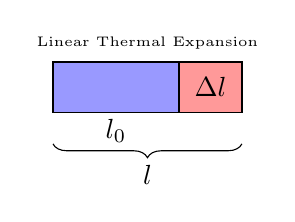
\begin{tikzpicture}[scale=0.8]
    \draw[fill=blue!40] (0,0) rectangle (2,0.8);
    \node at (1,-0.3) {$l_0$};
    \draw[fill=red!40] (2,0) rectangle (3,0.8);
    \node at (1.5,1.1) {\tiny Linear Thermal Expansion};
    \node at (2.5,0.4) {$\Delta l$};
    \draw [decorate,decoration={brace,amplitude=5pt,mirror}] (0,-0.5) -- (3,-0.5) node [black,midway,yshift=-0.4cm] {$l$};
\end{tikzpicture}
\end{column}
\end{columns}

\pagebreak
\item Surface thermal expansion
\vskip -15 pt
\begin{columns}
\begin{column}{0.6\textwidth}
\begin{eqnarray*}
\Delta A & \sim & A_0 \\
  \Delta A & \sim & \Delta T \\
  \Delta A & \sim & A_{0} \cdot \Delta T \\
  \Delta A & = & 2 \cdot \alpha \cdot A_0 \cdot \Delta T  \\
\Delta A & = & A - A_{0} \\
A & = & A_0 \cdot (1 + 2 \cdot \alpha \cdot \Delta T)
\end{eqnarray*}\\
$\alpha$: linear thermal expansion coefficient, $[\alpha] = 1/\text{K}$
\end{column}
\begin{column}{0.4\textwidth}
\vfill
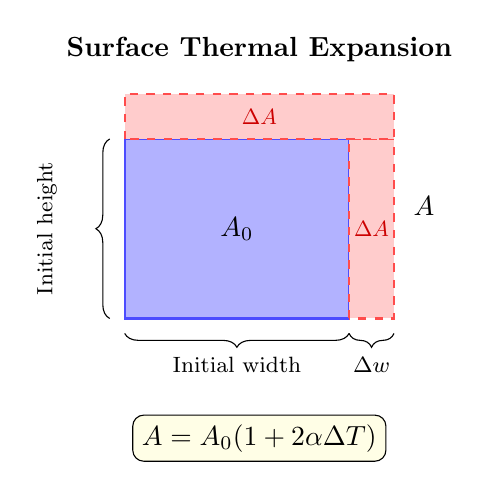
\begin{tikzpicture}[scale=1.9]
    % Az eredeti terület (kék téglalap)
    \draw[fill=blue!30, draw=blue!70, thick] (0,0) rectangle (1.5,1.2);
    \node at (0.75,0.6) {\textbf{$A_0$}};
    
    % A hőtágulás okozta növekmény (piros terület)
    \draw[fill=red!20, draw=red!70, thick, dashed] (1.5,0) rectangle (1.8,1.2);
    \draw[fill=red!20, draw=red!70, thick, dashed] (0,1.2) rectangle (1.8,1.5);
    
    % Feliratok a növekményekhez
    \node[red!80!black, scale=0.8] at (1.65,0.6) {$\Delta A$};
    \node[red!80!black, scale=0.8] at (0.9,1.35) {$\Delta A$};
    
    % Teljes terület jelölése (A)
    \node at (2,0.75) {\textbf{$A$}};
    
    % Méretek jelölése kapcsos zárójelekkel (angol feliratok)
    \draw [decorate,decoration={brace,amplitude=5pt,mirror}] (0,-0.1) -- (1.5,-0.1) 
        node [midway,yshift=-0.4cm] {\footnotesize Initial width};
        
    \draw [decorate,decoration={brace,amplitude=5pt,mirror}] (1.5,-0.1) -- (1.8,-0.1) 
        node [midway,yshift=-0.4cm] {\footnotesize $\Delta w$};

    \draw [decorate,decoration={brace,amplitude=5pt}] (-0.1,0) -- (-0.1,1.2) 
        node [midway,xshift=-0.8cm, rotate=90] {\footnotesize Initial height};

    % Cím
    \node[align=center, font=\bfseries] at (0.9,1.8) {Surface Thermal Expansion};
    
    % Képlet emlékeztetőnek
    \node[draw, fill=yellow!10, rounded corners] at (0.9,-0.8) {$A = A_0(1 + 2\alpha\Delta T)$};

\end{tikzpicture}
\end{column}
\end{columns}

\pagebreak
\item Volumetric thermal expansion
\vskip -15 pt
\begin{columns}
\begin{column}{0.6\textwidth}
  \begin{eqnarray*}
\Delta V & \sim & V_0 \\
\Delta V & \sim & \Delta T \\
\Delta V & \sim & V_{0} \cdot \Delta T \\  
\Delta V & = & 3\alpha \cdot V_0 \cdot \Delta T \\
\Delta V & = & V - V_0 \\ 
V & = & V_0 \cdot (1 + 3\alpha \cdot \Delta T) = V_0 \cdot (1 + \beta \cdot \Delta T)
\end{eqnarray*}
$\beta$: volumetric thermal expansion coefficient, $\beta = 3\alpha$
\end{column}
\begin{column}{0.4\textwidth}
\vfill
\begin{center}
% Izometrikus nézet beállítása
\tdplotsetmaincoords{70}{135}

\begin{tikzpicture}[tdplot_main_coords, scale=2.5]
    % Tengelyek (opcionális, elhagyható)
    %\draw[->] (0,0,0) -- (2,0,0) node[anchor=north east]{$x$};
    %\draw[->] (0,0,0) -- (0,2,0) node[anchor=north west]{$y$};
    %\draw[->] (0,0,0) -- (0,0,1.5) node[anchor=south]{$z$};

    % --- TÁGULT ÁLLAPOT (V) - Hátsó élek szaggatottal ---
    \draw[red!70, thick, dashed] (0,0,1.3) -- (1.3,0,1.3);
    \draw[red!70, thick, dashed] (0,1.3,1.3) -- (0,0,1.3);
    \draw[red!70, thick, dashed] (0,0,0) -- (0,0,1.3);

    % --- EREDETI ÁLLAPOT (V0) - Szilárd test ---
    % Alsó lap
    \draw[fill=blue!20, opacity=0.6] (0,0,0) -- (1,0,0) -- (1,1,0) -- (0,1,0) -- cycle;
    % Hátsó lapok
    \draw[fill=blue!30, opacity=0.6] (0,0,0) -- (0,0,1) -- (0,1,1) -- (0,1,0) -- cycle;
    \draw[fill=blue!30, opacity=0.6] (0,0,0) -- (1,0,0) -- (1,0,1) -- (0,0,1) -- cycle;
    % Első lapok
    \draw[fill=blue!40, opacity=0.6] (1,0,0) -- (1,1,0) -- (1,1,1) -- (1,0,1) -- cycle;
    \draw[fill=blue!40, opacity=0.6] (0,1,0) -- (1,1,0) -- (1,1,1) -- (0,1,1) -- cycle;
    % Felső lap
    \draw[fill=blue!50, opacity=0.6] (0,0,1) -- (1,0,1) -- (1,1,1) -- (0,1,1) -- cycle;
    
    \node at (0.5,0.6,0.7) {\textbf{$V_0$}};

    % --- TÁGULT ÁLLAPOT (V) - Első élek szilárd vonallal ---
    \draw[red!80, thick] (1.3,0,0) -- (1.3,1.3,0) -- (0,1.3,0);
    \draw[red!80, thick] (1.3,0,0) -- (1.3,0,1.3) -- (1.3,1.3,1.3) -- (1.3,1.3,0);
    \draw[red!80, thick] (0,1.3,0) -- (0,1.3,1.3) -- (1.3,1.3,1.3);

    % --- JELÖLÉSEK (Angolul) ---
    % Kezdő méret jelölése
    \draw[<->, blue!80!black] (0,0,-0.1) -- (1,0,-0.1) node[midway, below, sloped] {\tiny Initial length};
    
    % Tágulás jelölése
    \draw[<->, red!80!black] (1,0,-0.1) -- (1.3,0,-0.1) node[midway, below] {\tiny $\Delta L$};
    
    % Feliratok
    \node[anchor=west] at (1.4,0.5,0.7) {\textcolor{red!80!black}{\textbf{Volumetric Expansion}}};
    \node[anchor=west, scale=0.8] at (1.4,0.5,0.4) {\textcolor{blue!80!black}{$V_0$: Initial volume}};
    \node[anchor=west, scale=0.8] at (0.2,0.5,0.2) {\textcolor{red!80!black}{$V$: Expanded volume}};

    % Képlet
    \node[draw, fill=yellow!10, rounded corners] at (0.9, 1.8, 2.0) {$V = V_0(1 + 3\alpha\Delta T)$};

\end{tikzpicture}
\end{center}
\end{column}
\end{columns}

\end{itemize}

\end{frame}

% ----------------------------------------------------------------------------------------------------------------------------------------

\begin{frame}[fragile,squeeze,allowframebreaks]
\frametitle{Thermodynamics -- Thermometer}
\begin{itemize}
\item Bimetal
\vskip -20 pt  
\begin{columns}
\begin{column}{0.55\textwidth}
\begin{itemize}
    \item Based on thermal expansion
%    \item Solid-state thermometers
    \item The bending effect caused by the difference in thermal expansion of two materials with different material properties is used to measure temperature.
    \item Bimetellic thermometers use the bending effect caused by the difference in thermal expansion of the two metals to measure temperature.
    \item It is used to measure the effects of temperature change. The bimetal strip bends in response to changes in temperature
    \item Two different kinds of thermal expansions   
    \item Used for fire detection
\end{itemize}
\end{column}
\begin{column}{0.35\textwidth}
\vfill
\begin{center}
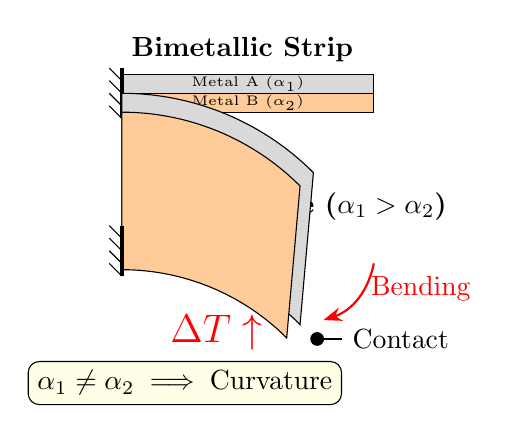
\begin{tikzpicture}[scale=0.8]

    % --- EREDETI ÁLLAPOT (Szobahőmérséklet) ---
    \node[anchor=west, font=\bfseries] at (0,2.5) {Bimetallic Strip};
    
    % Felső fém réteg
    \draw[fill=gray!30] (0,1.8) rectangle (4,2.1);
    \node at (2,1.95) {\tiny Metal A ($\alpha_1$)};
    
    % Alsó fém réteg
    \draw[fill=orange!40] (0,1.5) rectangle (4,1.8);
    \node at (2,1.65) {\tiny Metal B ($\alpha_2$)};
    
    % Falhoz rögzítés
    \draw[ultra thick] (0,1.4) -- (0,2.2);
    \foreach \y in {1.4, 1.6, 1.8, 2.0}
        \draw (0,\y) -- (-0.2, \y+0.2);

    % --- MELEGÍTETT ÁLLAPOT (Elhajlás) ---
    \begin{scope}[yshift=-2.5cm]
        \node[anchor=west, font=\bfseries] at (0,2.5) {Heated State ($\alpha_1 > \alpha_2$)};
        
        % Íves fémek rajzolása ( Metal A tágul jobban, ezért kívül van)
        % Metal A (felső/külső)
        \draw[fill=gray!30] (0,1.8) arc (90:45:4) -- (45:4.3) arc (45:90:4.3) -- cycle;
        
        % Metal B (alsó/belső)
        \draw[fill=orange!40] (0,1.5) arc (90:45:3.7) -- (45:4) arc (45:90:4) -- cycle;

        % Falhoz rögzítés
        \draw[ultra thick] (0,1.4) -- (0,2.2);
        \foreach \y in {1.4, 1.6, 1.8, 2.0}
            \draw (0,\y) -- (-0.2, \y+0.2);
            
        % Kapcsoló érintkező (Switch contact)
        \draw[fill=black] (3.1, 0.4) circle (0.1);
        \draw[thick] (3.1, 0.4) -- (3.5, 0.4) node[right] {Contact};
        
        % Nyíl az elhajlás jelzésére
        \draw[->, >=Stealth, bend left, red, thick] (4, 1.6) to (3.2, 0.7);
        \node[red, right] at (3.8, 1.2) {Bending};
        
        % Hő jelzése
        \node at (1.5, 0.5) {\Large \textcolor{red}{$\Delta T \uparrow$}};
    \end{scope}

    % Megjegyzés a hőtágulási együtthatókról
    \node[draw, fill=yellow!10, rounded corners] at (1,-2.8) {$\alpha_1 \neq \alpha_2 \implies \text{Curvature}$};

\end{tikzpicture}
\end{center}
\end{column}
\end{columns}

\pagebreak
\item Resistance thermometer
\begin{center}
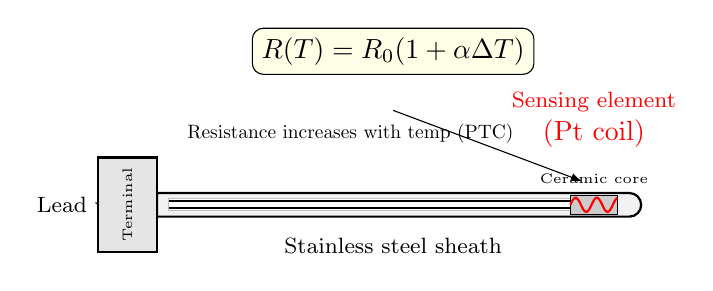
\begin{tikzpicture}[scale=1.5]
    % --- Védőburkolat (Protective Sheath) ---
    \draw[thick, fill=gray!10] (0,0.1) -- (4,0.1) arc (90:-90:0.1) -- (0,-0.1) -- cycle;
    \node[anchor=north] at (2,-0.2) {\footnotesize Stainless steel sheath};

    % --- Belső szigetelés (Insulation) ---
    \draw[fill=white, draw=gray!50] (0.1,0.05) rectangle (3.5,-0.05);

    % --- Kerámia mag (Ceramic Core) ---
    \draw[fill=gray!40] (3.5,0.08) rectangle (3.9,-0.08);
    \node[anchor=south] at (3.7,0.1) {\tiny Ceramic core};

    % --- Platina tekercs (Platinum Sensing Wire) ---
    % Szinuszos hullám a huzal jelképezésére
    \draw[red, thick] plot[domain=3.5:3.9, samples=50] (\x, {0.06*sin(2000*(\x-3.5))});
    \node[red, anchor=south, align=center] at (3.7, 0.4) {\footnotesize Sensing element \\ (Pt coil)};

    % --- Kivezető huzalok (Lead Wires) ---
    \draw[thick] (0.1, 0.03) -- (3.5, 0.03);
    \draw[thick] (0.1, -0.03) -- (3.5, -0.03);
    \node[anchor=east] at (0,0) {\footnotesize Lead wires};

    % --- Csatlakozó fej (Connection Head) vázlata ---
    \draw[thick, fill=gray!20] (-0.5,-0.4) rectangle (0,0.4);
    \node[rotate=90] at (-0.25,0) {\tiny Terminal};

    % --- Működési elv képlet ---
    \node[draw, fill=yellow!10, rounded corners] at (2, 1.3) {$R(T) = R_0 (1 + \alpha \Delta T)$};
    
    % --- Magyarázó nyilak ---
    \draw[->, >=latex] (2, 0.8) -- (3.6, 0.2);
    \node[anchor=west, scale=0.7] at (0.2, 0.6) {Resistance increases with temp (PTC)};
\end{tikzpicture}
\end{center}
\begin{itemize}
\item Based on thermal expansion
\item Solid-state thermometers
\item The resistance of a metal wire changes with temperature change
\item Platinum resistance thermometer: the changes of the resistance of the platinum is used for
temperature measurement
\item Wide range of linearity
  
\pagebreak
\item Two types of semiconductor solid-state thermometer:
\begin{itemize}
\item NTC (Negative Temperature Coefficient): as the temperature increases, the resistance of an NTC thermistor   decreases. This negative correlation between resistance and temperature gives it its name.
\item  PTC (Positive Temperature Coefficient): in contrast to NTC thermistors, the resistance of a PTC thermistor increases as the temperature rises. The positive correlation gives it its name.
\end{itemize}
\end{itemize}

\pagebreak
\item Liquid thermometers: Mercury or alcohol thermometer
\vskip -15 pt
\begin{columns}
\begin{column}{0.7\textwidth}
\begin{itemize}
\item Based on thermal expansion
\item Liquid thermometers: Mercury or alcohol thermometer
\item The liquid thermal expansion is used for temperature measurement
\item The thermometer has a uniformly spaced scale.
\item The alcohol is placed in an expansion vessel, which is connected to a capillary tube. The higher the temperature, the higher the alcohol rises in the capillary tube.
\item For example: traditional room thermometer
\end{itemize}
\end{column}
\begin{column}{0.2\textwidth}
\begin{center}
\includegraphics[width=0.5\textwidth]{images-20260309/thermometer.png}
\end{center}
\end{column}
\end{columns}


\pagebreak
\item Gas thermometers, Constant-pressure gas thermometer:
\vskip -15 pt
\begin{columns}
\begin{column}{0.3\textwidth}
\begin{itemize}
\item Based on thermal expansion
\item The has thermal expansion
\item The change in volume of the confined gas is read.
\item The mercury droplet rises in the thermometer as the temperature increases.
\end{itemize}
\end{column}
\begin{column}{0.6\textwidth}
\vfill
\begin{center}
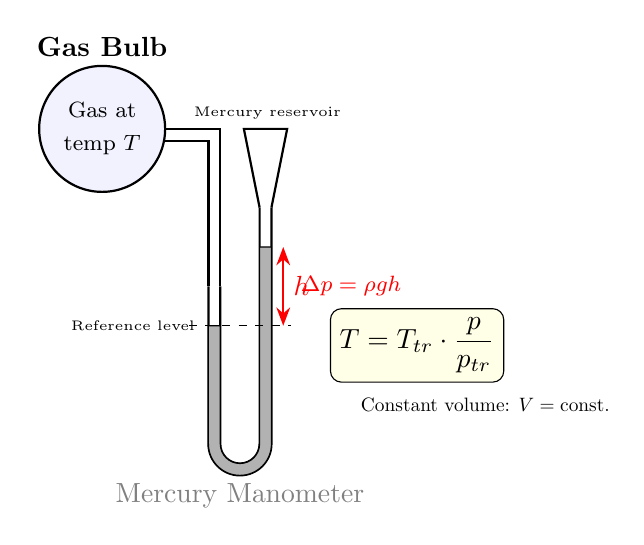
\begin{tikzpicture}[scale=1.0]

    % --- Gáztartály (Gas Bulb) ---
    \draw[thick, fill=blue!5] (0,0) circle (0.8);
    \node[align=center] at (0,0) {\footnotesize Gas at \\ \footnotesize temp $T$};
    \node[anchor=south] at (0,0.8) {\textbf{Gas Bulb}};

    % --- Összekötő cső ---
    \draw[thick] (0.8,0) -- (1.5,0) -- (1.5,-2);
    \draw[thick] (0.78,-0.15) -- (1.35,-0.15) -- (1.35,-2);

    % --- U-cső (Manométer) bal szár ---
    \draw[thick] (1.35,-2) -- (1.35,-4) arc(180:360:0.4) -- (2.15,-1);
    \draw[thick] (1.5,-2) -- (1.5,-4) arc(180:360:0.25) -- (2,-1);

    % --- Higanyszint (Mercury) ---
    % Bal oldali szint (referencia pont)
    \draw[fill=gray!60] (1.35,-2.5) -- (1.5,-2.5) -- (1.5,-4) arc(180:360:0.25) -- (2,-1.5) -- (2.15,-1.5) -- (2.15,-4) arc(360:180:0.4) -- cycle;
    
    % Jelzés a referencia szintnél
    \draw[dashed] (1.1,-2.5) -- (2.4,-2.5);
    \node[anchor=east] at (1.3,-2.5) {\tiny Reference level};

    % Magasságkülönbség (h) jelölése
    \draw[<->, >=Stealth, thick, red] (2.3,-2.5) -- (2.3,-1.5) node[midway, right] {$h$};
    \node[red, anchor=west] at (2.4,-2) {\footnotesize $\Delta p = \rho g h$};

    % --- Tartály a higanynak (Flexible tube / Reservoir) ---
    \draw[thick] (2,-1) -- (1.8,0) -- (2.35,0) -- (2.15,-1);
    \node[anchor=south] at (2.1,0) {\tiny Mercury reservoir};

    % --- Feliratok ---
    \node[anchor=north, gray] at (1.75,-4.375) {Mercury Manometer};
    
    % Képlet dobozban
    \node[draw, fill=yellow!10, rounded corners] at (4, -2.75) {
        $\displaystyle T = T_{tr} \cdot \frac{p}{p_{tr}}$
    };
    
    \node[anchor=west, scale=0.7] at (3.2, -3.5) {Constant volume: $V = \text{const.}$};

\end{tikzpicture}
\end{center}
\end{column}
\end{columns}

\pagebreak
\item Special thermometers
\vskip -15 pt
\begin{columns}
\begin{column}{0.7\textwidth}
\begin{itemize}
\item \textbf{Laser based thermometer:}
  \begin{itemize}
  \item Every object emits thermal radiation, the wavelength of which depends on the temperature of the objective.
  \item A major advantage is that there is no direct contact with the object being measured.
  \end{itemize}
\item \textbf{Colour thermometer:} e.g., used in metallurgy
%\end{itemize}
\end{itemize}
\end{column}
\begin{column}{0.2\textwidth}
\vfill
\begin{center}
\includegraphics[width=0.9\textwidth]{images-20260309/special_thermometer.png}
\end{center}
\end{column}
\end{columns}
  
\end{itemize}
\end{frame}

% ----------------------------------------------------------------------------------------------------------------------------------------

\begin{frame}[fragile,squeeze,allowframebreaks]
\frametitle{Phenomenological Thermodynamics}
\begin{itemize}  
\item State indicators
\begin{itemize}
    \item \textbf{Volume (V):} $[V] = m^3$
    \item \textbf{Pressure (p):} $[p) = Pa$
    \item \textbf{Temperature (T):} $[T] = K$
    \item \textbf{Amount of gas (n):} $ = mol$
\end{itemize}
\smallskip
\begin{center}
State indicators: p, V, T, n
\end{center}
\smallskip

\item \textbf{The ideal gas is a model:}
\vskip -20 pt
\begin{columns}
\begin{column}{0.7\textwidth}
\begin{itemize}
    \item Tiny, point-like particles (small spheres).
    \item Constant, random motion.
    \item Perfectly elastic collisions with each other and the walls.
    \item The volume of particles and long-range interactions are neglected.
    \item No attraction between gas particles.
\end{itemize}
\end{column}
\begin{column}{0.2\textwidth}
\vfill
\begin{center}
\includegraphics[width=1.2\textwidth]{images-20260309/idealgas.png}
\end{center}
\end{column}
\end{columns}

\pagebreak
\item The ideal gas equation of state
\begin{eqnarray*}
p \cdot V & = & n \cdot R \cdot T
\end{eqnarray*}
where p: pressure, V: volume, n: amount of substance (material), R: universal constant, T: temperature.
\item \textbf{Universal gas constant:} $R = 8.314 \frac{J}{mol \cdot K}$ \\
\item \textbf{Alternative forms:}
\begin{eqnarray*}
  p \cdot V & = & \frac{m}{M} \cdot R \cdot T\\
p \cdot V & = & m \cdot R_i \cdot T
\end{eqnarray*}
Where $M$ is molar mass, $m$ is mass, and $R_i = \frac{R}{M}$ is the individual gas constant.

\pagebreak
\item Special gas laws
  \vskip -10 pt
\begin{itemize}
\begin{columns}
\begin{column}{0.4\textwidth}
\item \textbf{Isothermal (T = const.):} Boyle – Mariotte Law: When the temperature of a given mass of confined gas is constant, the product of its pressure and volume is constant. During a state change at constant temperature (isotherm), the pressure and volume of an ideal gas are inversely proportional to each other.
\begin{eqnarray*}
p_1 \cdot V_1 & = & p_2 \cdot V_2
\end{eqnarray*}
\end{column}
\begin{column}{0.3\textwidth}
\vfill
\begin{center}
\includegraphics[width=0.9\textwidth]{images-20260309/bml.png}
\end{center}
\end{column}
\end{columns}

\pagebreak
\begin{columns}
\begin{column}{0.4\textwidth}
\item \textbf{Isobaric (p = const.):} Gay-Lussac I. Law: During a state change at constant pressure (isobaric), the volume and temperature of an ideal gas are directly proportional to each other; that is, the ratio of the volume to the temperature of the ideal gas is constant.
    \begin{eqnarray*}
    \frac{V_1}{T_1} & = & \frac{V_2}{T_2}
    \end{eqnarray*}
\end{column}
\begin{column}{0.3\textwidth}
\vfill
\begin{center}
\includegraphics[width=1.1\textwidth]{images-20260309/gll1.png}
\end{center}
\end{column}
\end{columns}
    
\pagebreak
\,
\vskip -20 pt
\begin{columns}
\begin{column}{0.4\textwidth}
\item \textbf{Isochoric (V = const.):} Gay-Lussac II. Law: During a state at constant volume (isochoric), the pressure and temperature of an ideal gas are directly proportional to each other; that is, the ratio of the pressure to the temperature of the ideal gas is constant
\begin{eqnarray*}
\frac{p_1}{T_1} & = & \frac{p_2}{T_2}
\end{eqnarray*}
\end{column}
\begin{column}{0.3\textwidth}
\vfill
\begin{center}
\includegraphics[width=1.1\textwidth]{images-20260309/gll2.png}
\end{center}
\end{column}
\end{columns}
\end{itemize}
\medskip
\item UNIVERSAL GAS LAW: If the amount of substance $n$ is constant:
\begin{eqnarray}
\frac{p_1 \cdot V_1}{T_1} & = & \frac{p_2 \cdot V_2}{T_2}
\end{eqnarray}
\end{itemize}    
\end{frame}

% ----------------------------------------------------------------------------------------------------------------------------------------

\begin{frame}[fragile,squeeze,allowframebreaks]
\frametitle{Heat, Specific Heat, Heat Capacity}
\begin{itemize}  
\item Joseph Black (1728-1799) Experiments and observations on heat processes.
\begin{itemize}
\item Heating a piece of copper and water on the same heating source (with the same surface area, same heat transfer), they reach different temperature in the same amount of time.
\item Different materials behave differently under the same amount of heat.
\item Heat has quantity.
\end{itemize}
\item Materials in contact with each other: \textbf{Heat flows, transfers from one material to another}
\vskip -80 pt
\begin{center}
\includegraphics[width=0.5\textwidth]{images-20260309/heatflow.png}
\end{center}
\vfill
  
\pagebreak
\item \textbf{Specific heat ($c$):} The heat required to raise the temperature of 1 kg of substance by $1^\circ C$.
\vskip -40 pt
\begin{eqnarray*}
Q & = & c \cdot m \cdot \Delta T \\
c & = & \frac{Q}{m \cdot \Delta T} \\
c & = & \frac{J}{kg \cdot {}^\circ C} = \frac{J}{kg \cdot K}
\end{eqnarray*}
\item Specific heat of ideal gases \\
Relationship: $c_p - c_V = R$
\begin{center}
\renewcommand{\arraystretch}{1.2}
\begin{tabular}{|l|c|c|}
\hline
\textbf{Type of gas} & $c_V$ & $c_p$ \\ \hline
One-atomic gases (He, Ne, Ar, Kr, Xe, \dots) – noble gases & $\frac{3}{2}R$ & $\frac{5}{2}R$ \\ \hline
Two-atomic gases ($H_{2}$, $O_{2}$, $N_{2}$, \dots)& $\frac{5}{2}R$ & $\frac{7}{2}R$ \\ \hline
More-atomic gases ($CH_{4}$, \dots) & $\frac{7}{2}R$ & $\frac{9}{2}R$ \\ \hline
\end{tabular}
\renewcommand{\arraystretch}{1}
\end{center}

\smallskip
\item \textbf{Heat Capacity:} The numerical value of the heat capacity indicates how much heat is required to raise the temperature of the body by 1 C degree. Symbol: K, dimension: J/K, J/$C^{\circ}$.
\vskip -30 pt
\begin{eqnarray*}
K & = & \frac{Q}{\Delta T} = c \cdot m \\
K & = & \frac{J}{K} = \frac{J}{^\circ C}
\end{eqnarray*}

\end{itemize}    
\end{frame}

% ----------------------------------------------------------------------------------------------------------------------------------------

\begin{frame}
%\frametitle{Minden jó, ha a vége jó}

\vfill
\begin{center}
\textbf{\huge The End}

\bigskip
Thank you for your attention!
\end{center}
\vfill
\textbf{Acknowledgements} Thank you for the course materials for Szilárd~ZSÓKA and Zoltán~VARGA.
\end{frame}

\end{document}
